\section{Test Cases}
\label{sec:results}

We analyze a series of two-dimensional cases to assess accuracy,
quantify artifacts introduced by the convex approximations, and gain
intuition into the physics and numerics.

For all cases, we use $v_s=10^{-4}\text{ m}/\text{s}$ for Lagged and Similar,
and $\sigma=10^{-3}$ for SAP, leading to very tight stiction modeling as
required for simulating manipulation tasks.

We estimate contact stiffness using Hertz theory. For a sphere of mass $m$ and
radius $R$, Hertz theory predicts a penetration
$\delta=(3mg/(4ER^{1/2}))^{2/3}$. For steel with Young's modulus $E=200\text{
GPa}$ and using the radii and masses from Sections \ref{sec:falling_sphere} and
\ref{sec:sliding_rod}, we obtain penetrations around $\delta\approx
2.5\times10^{-7}\text{ m}$ and stiffnesses $k\approx 1\times
10^{7}-2\times 10^{7}\text{ N}/\text{m}$. We use $k = 10^{7}\text{
N}/\text{m}$ for all cases in this section.

For some cases, we perform a convergence study where we compute the
error in the positions $\mf{q}_{\delta t}$ obtained using step size $\delta t$
against a reference $\mf{q}_\text{ref}$ as a function of the time step size
\begin{equation*}
    e_q(\delta t) = \left(\frac{1}{T}\int_0^T dt\Vert\mf{q}_{\delta t}(t)-\mf{q}_\text{ref}(t)\Vert^2\right)^{1/2}
\end{equation*}
where $T$ is simulation duration. The reference solution is obtained numerically
using a time step 10 times smaller than the smallest time step in the
convergence study. Since Lagged is the only approximation that is consistent
(Section \ref{sec:consistency}), we use it to compute the reference solution.

\subsection{Oscillating Conveyor Belt}

This test illustrates artifacts in the strongly coupled SAP and Similar
approximations. A $1 \text{ kg}$ box with $5\text{ cm}$ sides is placed on a
conveyor belt oscillating at $1 \text{ Hz}$ with $0.2 \text{ m}$ amplitude (Fig.
\ref{fig:belt_shematic}). Friction is $\mu=0.7$. Even though dissipation models
are different, using $d=500 \text{ s/m}$ for Similar and Lagged and
$\tau_d=10^{-3} \text{ s}$ for SAP yields comparable dissipation.

\begin{figure}[!h]
    \centering
    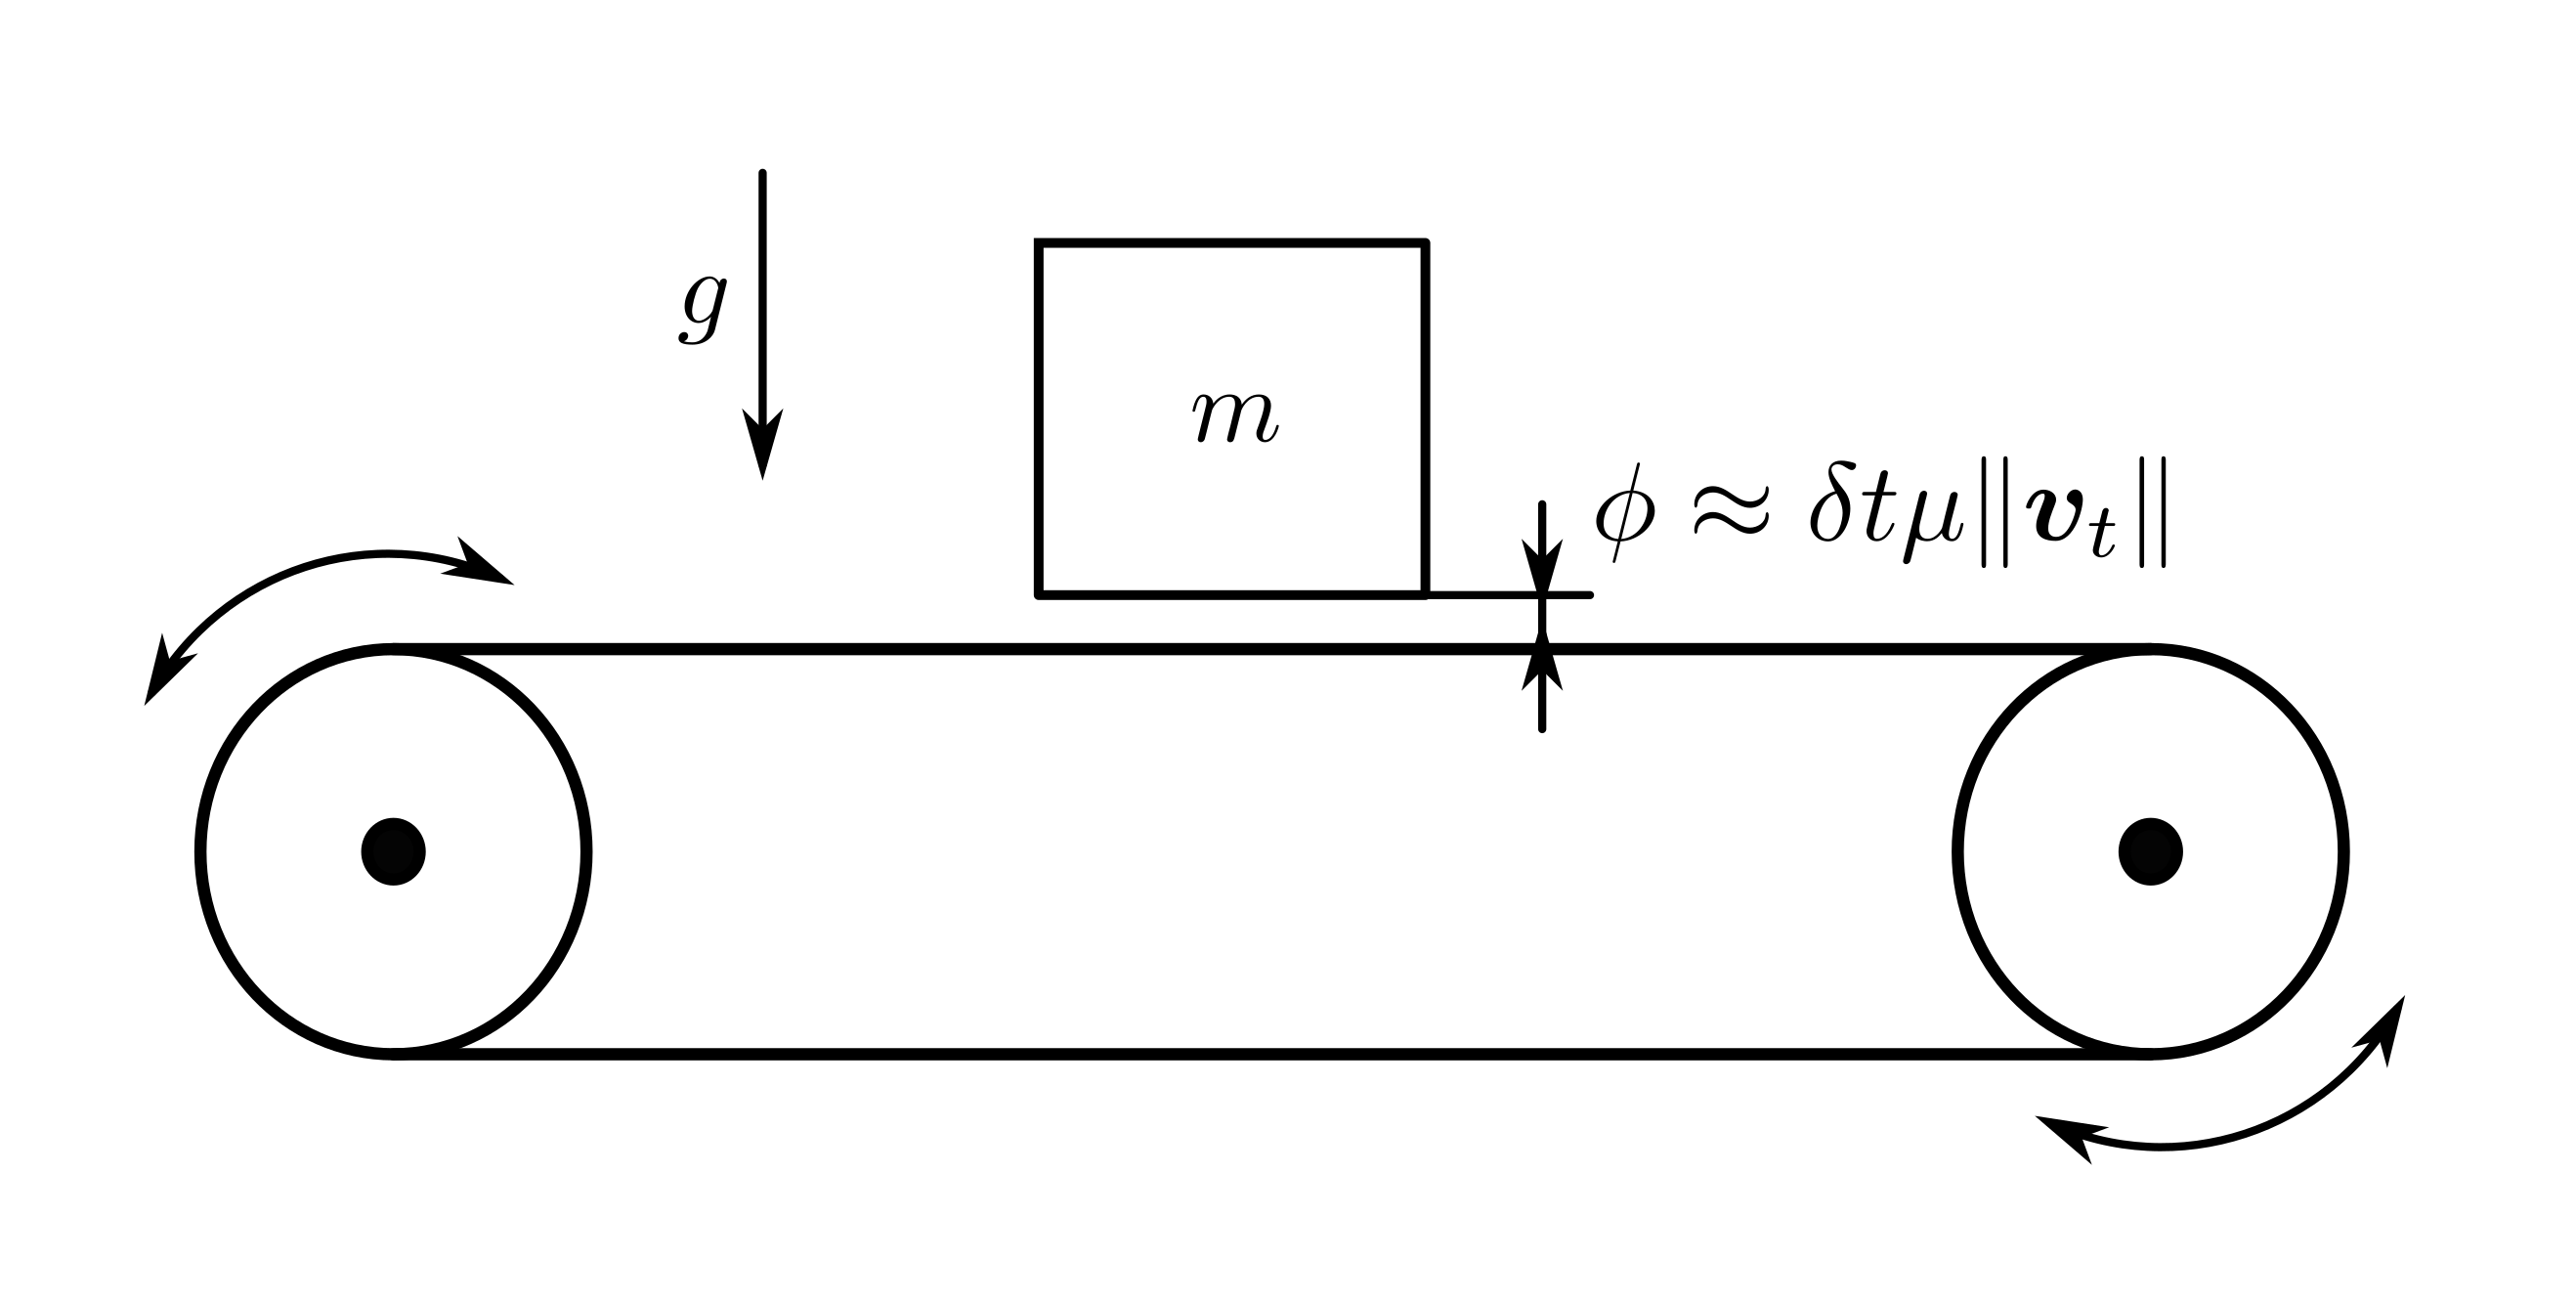
\includegraphics[width=0.8\columnwidth]{figures/TestCases/Belt/belt_schematics.png}
    \caption{Oscillating Conveyor Belt. SAP and Similar introduce artificial
    \emph{gliding} during slip phases (Section \ref{sec:gliding_artifact}).}
    \label{fig:belt_shematic}
\end{figure}

Figure \ref{fig:belt_contact_velocity_and_force} shows contact velocity and
force computed using $\delta t=0.01\text{ s}$. Contact between the box and belt
transitions back and forth between stiction and sliding. The Lagged
approximation predicts no vertical motion, with the normal force balancing the
box's weight as expected. However, SAP and Similar models show artifacts in the
normal direction during sliding, with non-zero normal velocity due to the
\emph{gliding} artifact, which disappears in stiction. Additionally, we observe
spurious transients in the normal force during sliding --- as slip speed changes
so does \emph{gliding}, causing vertical acceleration and thus normal force
fluctuations. Finally, SAP and Similar introduce normal force spikes
during the abrupt transition from sliding to stiction, when gliding vanishes
causing a sudden normal velocity change (Fig.
\ref{fig:belt_contact_velocity_and_force}).

\begin{figure}[!h]
    \centering
    %trim={<left> <lower> <right> <upper>}
    \adjincludegraphics[width=0.49\columnwidth,trim={0 0 {0.05\width} 0},clip]{figures/TestCases/Belt/contact_velocity_dt0p01.png}
    \adjincludegraphics[width=0.49\columnwidth,trim={0 0 {0.05\width} 0},clip]{figures/TestCases/Belt/contact_force_dt0p01.png}
    \caption{\label{fig:belt_contact_velocity_and_force} Contact velocity (left)
    and force (right). $\delta t=0.01\text{ s}$.}
\end{figure}

Figure \ref{fig:bel_convergence_position} shows a convergence study with step
sizes $\delta t \in \{2\times10^{-3}, 10^{-2}, 5\times10^{-2}\}$. Both Lagged
and Similar exhibit first order convergence, as expected, though the artifacts
introduced by Similar (Fig. \ref{fig:belt_contact_velocity_and_force}), cause
higher errors than Lagged. Finally, SAP's error plateaus at the smallest time
step due to model inconsistency, where the term $\tau_d\mu\Vert\vf{v}_t\Vert$ in
\eqref{eq:sap_gliding_offset} does not vanish as time step decreases.

\begin{figure}[!h]
    \centering
    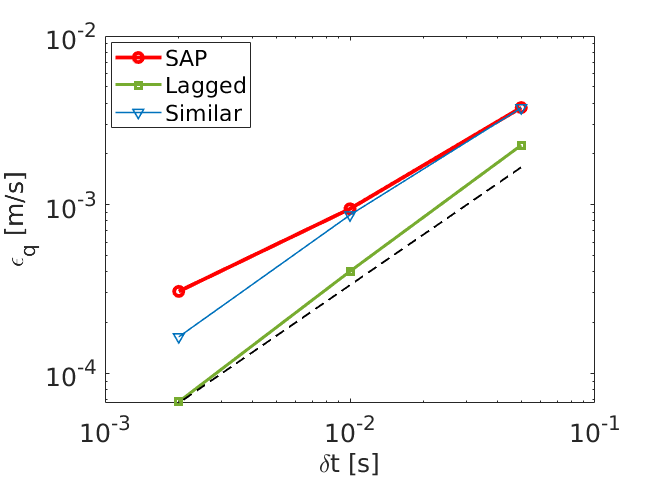
\includegraphics[width=0.8\columnwidth]{figures/TestCases/Belt/convergence_position.png}
    \caption{Convergence of the box trajectory with time step size. The dashed line is a reference for first order convergence.}
    \label{fig:bel_convergence_position}
\end{figure}


\subsection{Falling Sphere}
\label{sec:falling_sphere}

The conveyor belt case from the previous section favors the Lagged model due to
the steady-state normal force, where the Lagged model is exact. Here, we
introduce a collision test to evaluate approximations under sudden contact
force changes.

In this test, a $0.5\text{ kg}$ steel sphere $5\text{ cm}$ in diameter falls
from a height of $5\text{ cm}$ with an initial horizontal velocity $U_0=2\text{
m/s}$, see Fig. \ref{fig:sphere_schematic}. Friction with the ground is
$\mu=0.5$. Upon impact, the sphere slides, and then transitions to rolling
as friction induces angular momentum. After this transition, friction ceases to
dissipate energy. We model compliant contact with stiffness $k=10^{7}\text{
N/m}$ and dissipation constants $d=500\text{ s/m}$ and
$\tau_d=10^{-3}\text{ s}$.

\begin{figure}[!h]
    \centering
    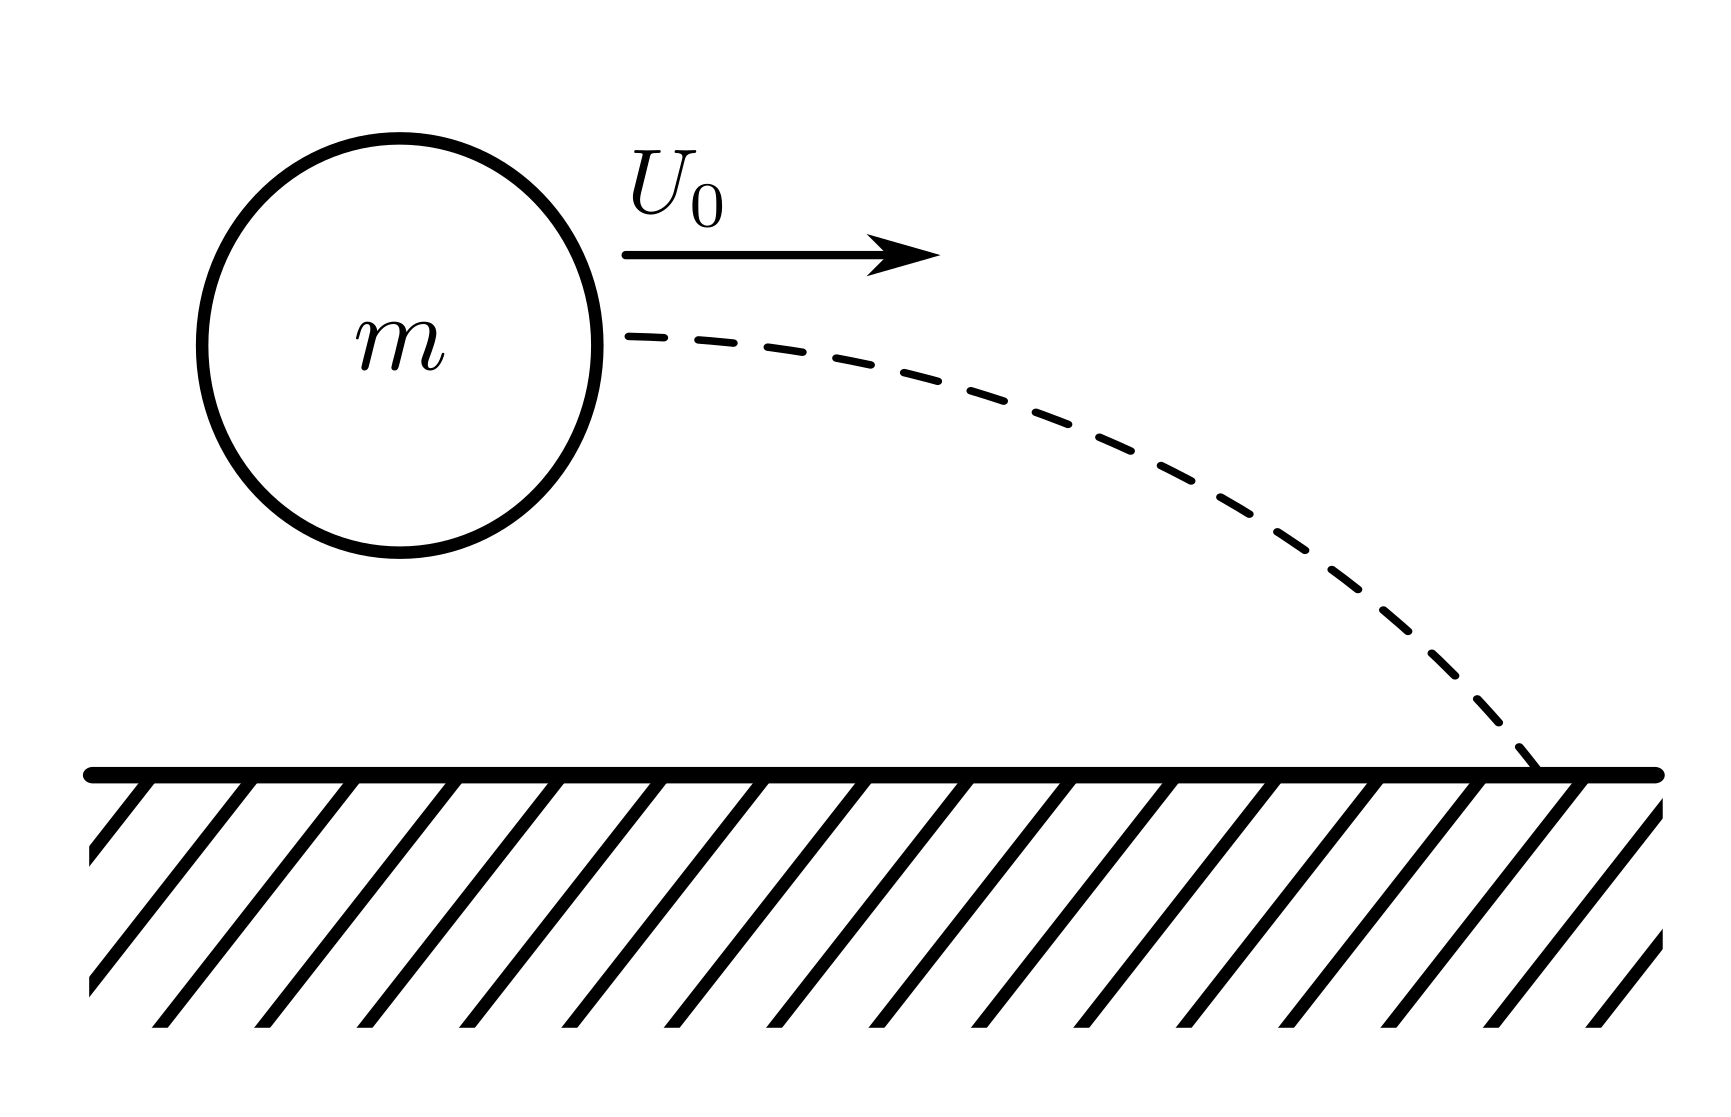
\includegraphics[width=0.6\columnwidth]{figures/TestCases/Cylinder/sphere_schematic.png}
    \caption{Falling sphere. After free fall, the sphere slides until friction with the ground establishes a rolling contact.}
    \label{fig:sphere_schematic}
\end{figure}

Figure \ref{fig:cylinder_contact_velocity_and_force} shows contact velocity and
force computed with $\delta t=2\times10^{-3}\text{ s}$. In the force plots, both
SAP and Similar initiate contact earlier due to the \emph{action at a distance}
artifact in these convex models, with SAP engaging even earlier due to the
non-vanishing term $\tau_d\mu\Vert\vf{v}_t\Vert$ in
\eqref{eq:sap_gliding_offset}. The sphere slides from initial contact until
about $t=0.07\text{ s}$, when it transitions to rolling. While Lagged brings
normal velocity to zero almost instantly, SAP and Similar models link normal
velocity to slip velocity, only reaching zero at stiction. During the
sliding-to-stiction transition, we observe a rapid normal force spike, as with
the conveyor belt problem. This artifact is absent with the Lagged
approximation.

\begin{figure}[!h]
    \centering
    %trim={<left> <lower> <right> <upper>}
    \adjincludegraphics[height=0.38\columnwidth,trim={0 0 {0.05\width} 0},clip]{figures/TestCases/Cylinder/contact_velocity_dt2em3.png}
    \adjincludegraphics[height=0.38\columnwidth,trim={0 0 {0.05\width} 0},clip]{figures/TestCases/Cylinder/contact_force_dt2em3.png}
    \caption{\label{fig:cylinder_contact_velocity_and_force} Contact velocity (left)
    and force (right) with $\delta t=2\times10^{-3}\text{ s}$.}
\end{figure}

A convergence study with step sizes $\delta t \in \{4\times10^{-4},
2\times10^{-3}, 10^{-2}\}$ is shown in Fig.
\ref{fig:cylinder_convergence_position}. While all of these schemes are first
order, SAP exhibits a constant error at convergence due to the
$\tau_d\mu\Vert\vf{v}_t\Vert$ term in \eqref{eq:sap_gliding_offset}.

\begin{figure}[!h]
    \centering
    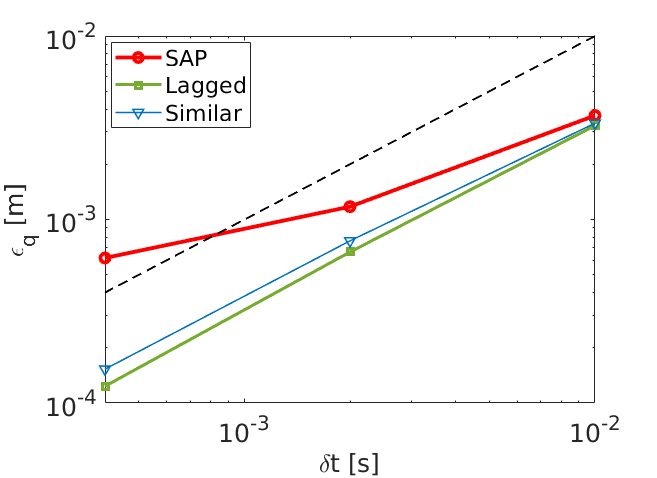
\includegraphics[width=0.8\columnwidth]{figures/TestCases/Cylinder/position_convergence.png}
    \caption{Convergence of the sphere trajectory with time step size. The dashed line is a reference for first order convergence.}
    \label{fig:cylinder_convergence_position}
\end{figure}


\subsection{Sliding Rod}
\label{sec:sliding_rod}

This case is particularly interesting as it leads to impact without collision
\cite[\S 5.3]{bib:pfeiffer1996multibody}. A rod initially angled with the ground
makes single-point contact with a horizontal velocity (see Fig.
\ref{fig:sliding_rod_setup}). As it slides, friction rotates the rod into the
ground, increasing the normal force. Under specific conditions, both normal and
frictional forces intensify, potentially leading to a singularity in
acceleration-level formulations with Coulomb friction known as Painlev\'e's
paradox, where forces become infinite. This problem is resolved in the discrete
setting, where finite impulses and discrete velocity changes are allowed.
Physically, bodies aren't perfectly rigid --- they deform, vibrate, and may
even undergo plastic (permanent) deformations. Nonetheless, a rapidly increasing
contact force develops an impact that makes the rod jam into the ground and jump
into the air. The rod measures $0.5\text{ m}$ in length, $1\text{ cm}$ in
diameter, and has a mass of $0.3\text{ kg}$.

\begin{figure}[!h]
    \centering
    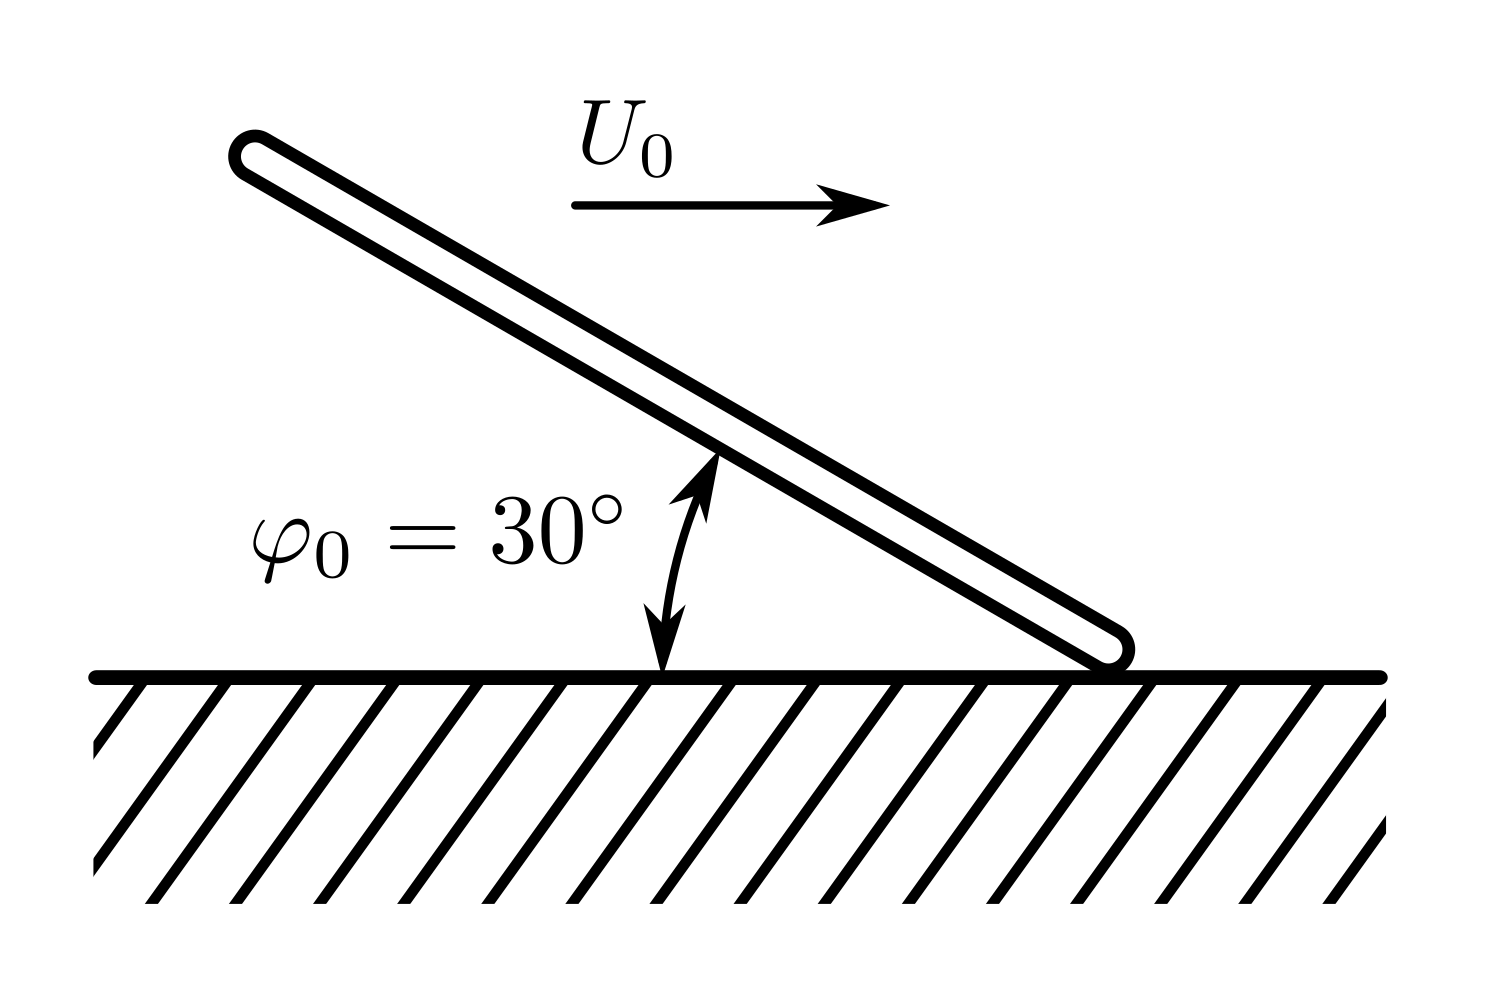
\includegraphics[width=0.55\columnwidth]{figures/TestCases/SlidingRod/sliding_rod_schematic.png}
    \caption{Sliding rod. Initially forming an angle $\varphi_0$ with the ground
    and with horizontal velocity $U_0$. Friction makes the rod rotate clockwise.
    The contact force increases until the rod jams into the ground, causing the
    rod to jump into the air.}
    \label{fig:sliding_rod_setup}
\end{figure}

Analytical analysis \cite[\S 5.3]{bib:pfeiffer1996multibody} shows that the
singularity occurs when $\mu>4/3$ and the initial kinetic energy overcomes
potential energy as the rod's center of gravity rises and friction dissipates
energy. We set $\mu=2.3$, a $30^\circ$ initial angle (Fig.
\ref{fig:sliding_rod_setup}), and an initial horizontal speed $U_0=10\text{
m}/\text{s}$.

Using a reference solution with a time step of $\delta t=10^{-7}\text{ s}$ and no
normal force dissipation, we observe that the rod rotates upward and jams into
the ground upon contact as expected. All three models yield similar results, as
the compliant model is identical in the absence of dissipation, differing only
in friction regularization. Pre-impact forces oscillate based on ground
compliance, and impact location is nearly identical across models (
Fig. \ref{fig:rod_contact_force_no_diss}) despite being very sensitive to model
parameters.

\begin{figure}[!h]
    \centering
    %trim={<left> <lower> <right> <upper>}
    \adjincludegraphics[height=0.375\columnwidth,trim={0 0 {0.05\width} 0},clip]{figures/TestCases/SlidingRod/SteelRod/contact_forces_no_diss.png}
    \adjincludegraphics[height=0.375\columnwidth,trim={0 0 {0.05\width} 0},clip]{figures/TestCases/SlidingRod/SteelRod/contact_forces_no_diss_zoom.png}
    \caption{\label{fig:rod_contact_force_no_diss} Contact forces in the case with zero
    dissipation. The figure on the right shows a close-up near the impact.}
\end{figure}

Figure \ref{fig:rod_contact_velocity_no_diss} shows the contact point moves
into the ground due to large contact forces until the tangential component of
the velocity goes to zero and the rod jams into the ground. During stiction
$\Vert\vf{v}_t\Vert<v_s$ for a finite period of about $0.2\text{ ms}$.

\begin{figure}[!h]
    \centering
    %trim={<left> <lower> <right> <upper>}
    \adjincludegraphics[height=0.375\columnwidth,trim={0 0 {0.05\width} 0},clip]{figures/TestCases/SlidingRod/SteelRod/contact_velocities_no_diss.png}
    \adjincludegraphics[height=0.375\columnwidth,trim={0 0 {0.05\width} 0},clip]{figures/TestCases/SlidingRod/SteelRod/contact_velocities_no_diss_zoom.png}
    \caption{\label{fig:rod_contact_velocity_no_diss} Contact velocities in the case with zero
    dissipation. The figure on the right shows a close-up near the impact.}
\end{figure}

We run the simulation with Hunt \& Crossley dissipation $d=0.2\text{ s}/\text{m}$
and relaxation time $\tau_d = 4.0\times{10}^{-6}\text{ s}$. These low
dissipation values have minimal effect on the time of impact for the Lagged model,
our reference solution, as seen in Figs. \ref{fig:rod_contact_force} and
\ref{fig:rod_contact_velocity}. However, Similar and SAP models predict shifted
impact times—earlier for Similar, later for SAP. Although their contact forces and
velocities differ significantly, we choose $\tau_d$ for SAP to match the shift in time
of impact observed in the Similar model, albeit in the opposite direction.
Compliance modulation in Similar becomes evident in Fig.
\ref{fig:rod_contact_force}, where we observe a frequency shift on the force
oscillations. This is caused by the larger effective stiffness of the model
during sliding, $k_\text{eff}=k\,(1+\mu\Vert\vf{v}_t\Vert\,d)$.

\begin{figure}[!h]
    \centering
    %trim={<left> <lower> <right> <upper>}
    \adjincludegraphics[height=0.375\columnwidth,trim={0 0 {0.05\width} 0},clip]{figures/TestCases/SlidingRod/SteelRod/contact_forces.png}
    \adjincludegraphics[height=0.375\columnwidth,trim={0 0 {0.05\width} 0},clip]{figures/TestCases/SlidingRod/SteelRod/contact_forces_zoom.png}
    \caption{\label{fig:rod_contact_force} Contact forces in the case
    with dissipation. The figure on the right shows a close-up near the impact.}
\end{figure}

A convergence analysis with and without dissipation is shown in Fig.
\ref{fig:rod_convergence}, using time steps $\delta t=\{6.4\times 10^{-4},
1.6\times 10^{-4}, 4.0\times 10^{-5}, 1.0\times 10^{-5}\}\text{ s}$. Without
dissipation, SAP and Similar model solutions are indistinguishable. The Lagged
model exhibits the largest error at the largest time step. revealing a limitation:
its lagged normal force affects Coulomb friction modeling in rapidly changing
scenarios, even missing impacts when $\delta t > 10^{-3}\text{ s}$. However, it
achieves first-order convergence with smaller steps. Similar trends occur with
non-zero dissipation, though the curves diverge as time of impact predictions shift.

\begin{figure}[!h]
    \centering
    %trim={<left> <lower> <right> <upper>}
    \adjincludegraphics[height=0.375\columnwidth,trim={0 0 {0.05\width} 0},clip]{figures/TestCases/SlidingRod/SteelRod/contact_velocities.png}
    \adjincludegraphics[height=0.375\columnwidth,trim={0 0 {0.05\width} 0},clip]{figures/TestCases/SlidingRod/SteelRod/contact_velocities_zoom.png}
    \caption{\label{fig:rod_contact_velocity} Contact velocities in the case
    with dissipation. The figure on the right shows a close-up near the impact.}
\end{figure}


\begin{figure}[!h]
    \centering
    %trim={<left> <lower> <right> <upper>}
    \adjincludegraphics[height=0.375\columnwidth,trim={0 0 {0.05\width} 0},clip]{figures/TestCases/SlidingRod/SteelRod/position_errors_no_diss.png}
    \adjincludegraphics[height=0.375\columnwidth,trim={0 0 {0.05\width} 0},clip]{figures/TestCases/SlidingRod/SteelRod/position_errors.png}
    \caption{\label{fig:rod_convergence} Convergence in positions with
    time step. Case without dissipation (left) and with dissipation (right).}
\end{figure}

